\part{Arithmetic Logic Unit}
\frame{\partpage}

\begin{frame}{Arithmetic Logic Unit}
	\begin{center}
		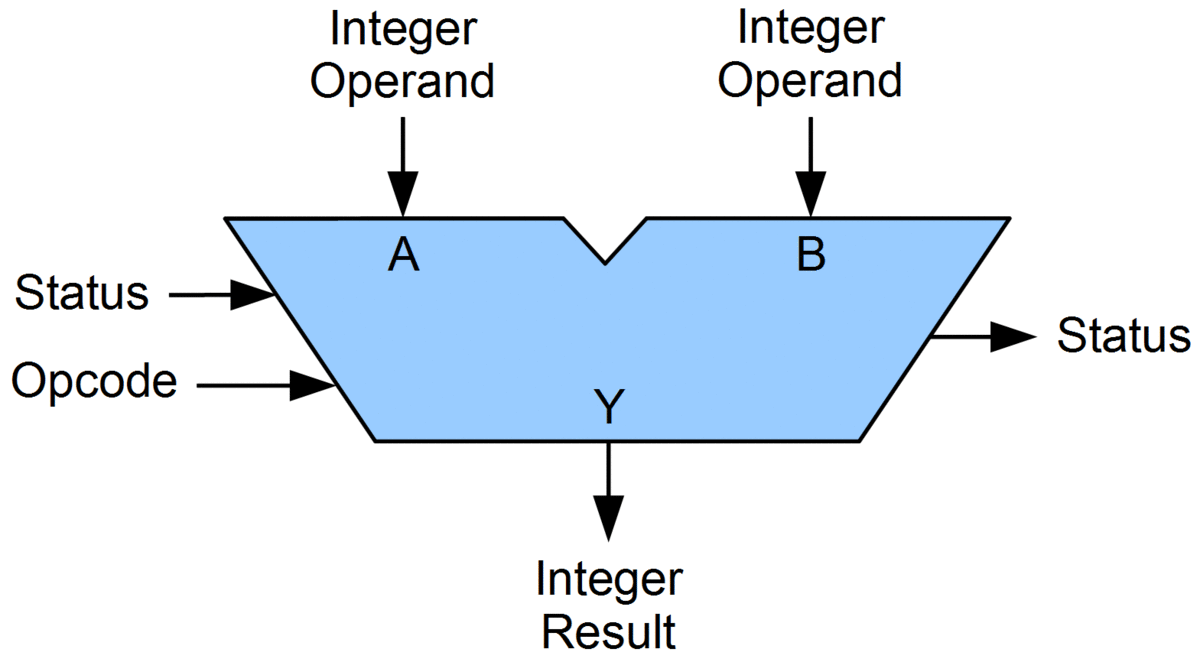
\includegraphics[width=\textwidth]{alu}
		%https://commons.wikimedia.org/wiki/File:ALU_block.gif
	\end{center}
\end{frame}

\begin{frame}{Arithmetic Logic Unit}
	\begin{itemize}
		\pause\item Important part of the CPU
		\pause\item Inputs:
			\begin{itemize}
				\item \textbf{Operand} words $A, B$
				\item \textbf{Opcode}
				\item \textbf{Status} bits
			\end{itemize}
		\pause\item Outputs:
			\begin{itemize}
				\item \textbf{Result} word $Y$
				\item \textbf{Status} bits
			\end{itemize}
		\pause\item Opcode specifies how $Y$ is calculated based on $A$ and $B$
	\end{itemize}
\end{frame}

\begin{frame}{ALU operations}
	Typically include:
	\begin{itemize}
		\pause\item Add with carry
		\pause\item Subtract with borrow
		\pause\item Negate (2's complement)
		\pause\item Increment, decrement
		\pause\item Bitwise \textsc{and}, \textsc{or}, \textsc{not}, $\dots$
		\pause\item Bit shifts
	\end{itemize}
\end{frame}

\newcommand{\carry}[1]{\uncover<#1->{$_1$}}
\newcommand{\nocarry}[1]{\phantom{$_1$}}

\begin{frame}{Addition with carry}
	In base 10:
	\begin{center}
		\begin{tabular}{lllll}
			& 1 & 2 & 3 & 4 \\
			+ & 5\nocarry{4} & 6\carry{3} & 7\carry{2} & 8\nocarry{1} \\\hline
			& \uncover<5->{6} & \uncover<4->{9} & \uncover<3->{1} & \uncover<2->{2}
		\end{tabular}
	\end{center}
\end{frame}

\begin{frame}{Addition with carry}
	In base 2:
	\begin{center}
		\fbox{$1 + 1 = 10$ \qquad $1 + 1 + 1 = 11$}
		
		\vspace{2ex}
		
		\begin{tabular}{lllllllll}
			& 0 & 1 & 1 & 0 & 1 & 1 & 1 & 0 \\
			+ &
				0\carry{8} &
				0\carry{7} &
				1\nocarry{6} &
				0\carry{5} &
				0\carry{4} &
				1\carry{3} &
				1\nocarry{2} &
				1 \\\hline
			&
				\uncover<9->{1} &
				\uncover<8->{0} &
				\uncover<7->{0} &
				\uncover<6->{1} &
				\uncover<5->{0} &
				\uncover<4->{1} &
				\uncover<3->{0} &
				\uncover<2->{1}
		\end{tabular}
	\end{center}
\end{frame}

\begin{frame}{1-bit adder}
	\begin{center}
		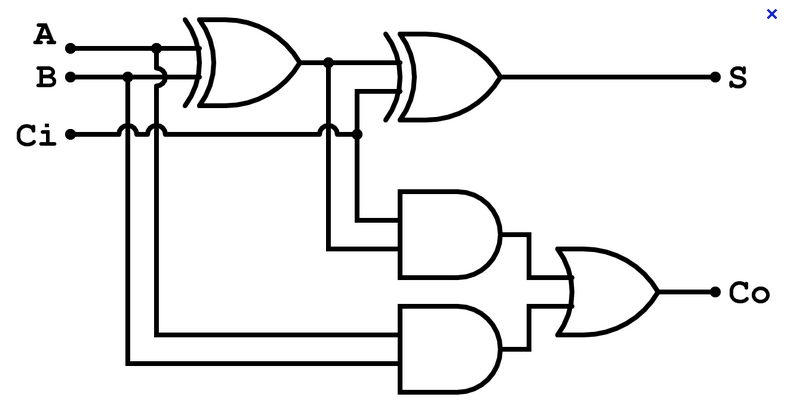
\includegraphics[width=\textwidth]{1bit_adder}
	\end{center}
\end{frame}

\begin{frame}{$n$-bit adder}
	\begin{center}
		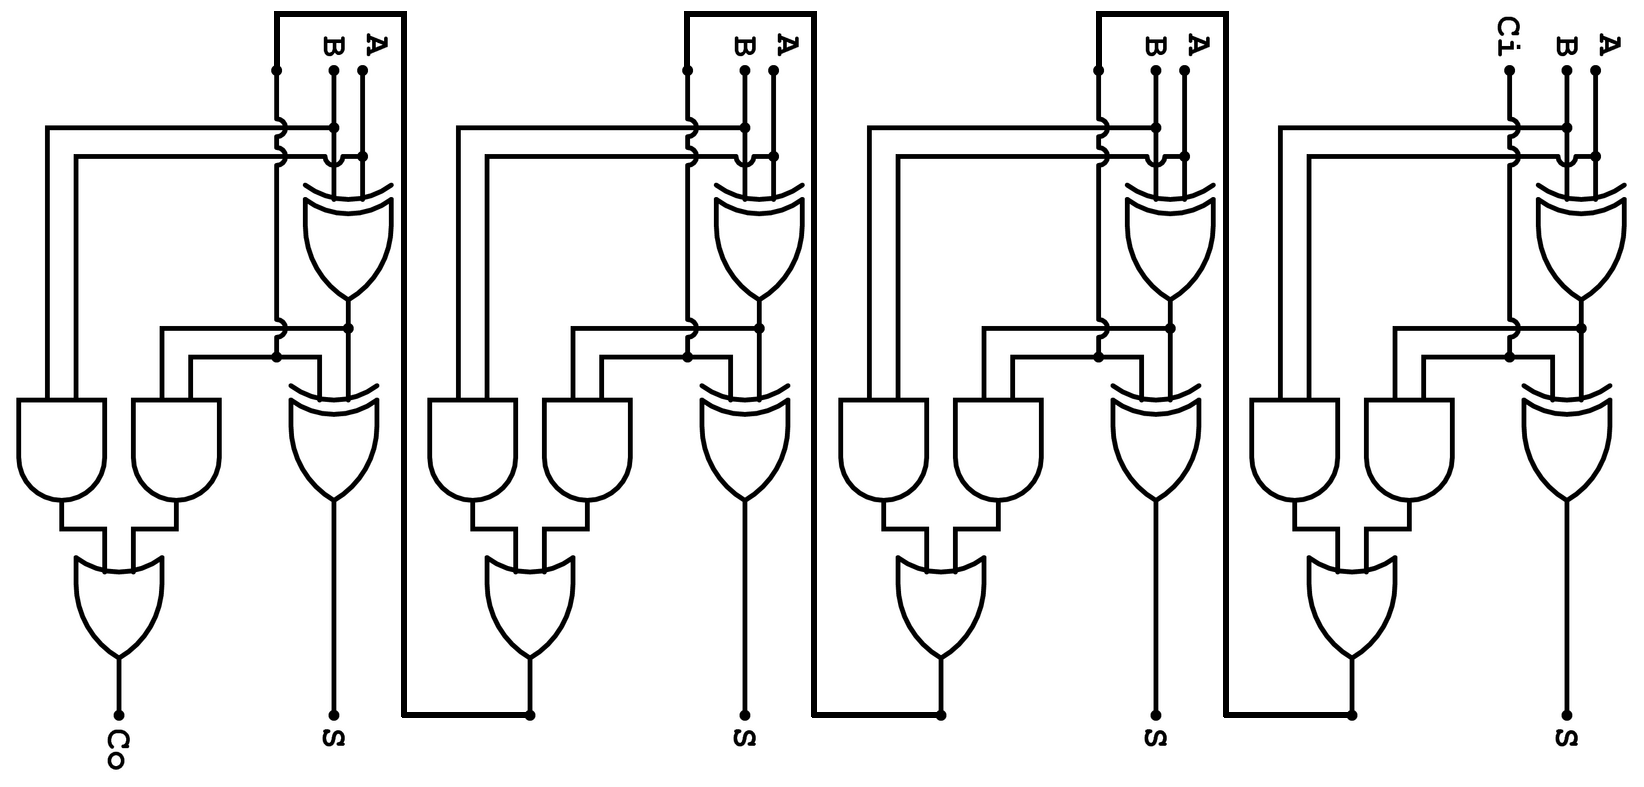
\includegraphics[width=\textwidth]{nbit_adder}
	\end{center}
\end{frame}

